Despite the conceivable advantages of \ac{NVRAM}, there are also challenges to
be addressed. Although most issues are of practical nature there are also
conceptual concerns.

\subsection{Unintended Durability}

The key feature of \ac{NVRAM} is to retain its data across restarts. However,
not all data is necessarily intended to be durable. Notable examples include
transient, confidential, and corrupt data. The former comprises data which may
not be valid after a system restart, as is the case with data related to machine
or device state.

\paragraph{Information Security}

% Other data such as passwords, encryption keys, or decrypted data may be
% confidential and should not be durable. It has been shown that even volatile
% \ac{RAM} holds its charge long enough so that a module can be moved to an
% attacker's machine for read-out \cite{halderman2008lest}. Despite being
% countered with hardware scramblers, researchers still managed to apply
% variations of the technique and obtain vital information
% \cite{yitbarek2017cold}. Such attacks would be trivial on \ac{NVRAM}
% \cite{bailey2011operating}, but that is beyond the scope of this work.
Other data such as passwords, encryption keys, or decrypted data may be
confidential and should not be durable. It has been shown that even volatile
\ac{RAM} holds its charge long enough so that a module can be moved to an
attacker's machine for read-out \cite{halderman2008lest, yitbarek2017cold}. Such
attacks would be trivial on \ac{NVRAM} \cite{bailey2011operating}, but that is
beyond the scope of this work.

% By cooling the module, capacitor
% discharge can be slowed so that it can be moved to another machine where its
% content may be read and parsed. Despite being countered with hardware
% scramblers, researchers still managed to apply variations of the technique and
% obtain vital information \cite{yitbarek2017cold}. Such attacks would be trivial
% on \ac{NVRAM}, as durability is its primary feature \cite{bailey2011operating}. Of
% course, confidential data could be overwritten with zeros after usage, but there
% is always a possibility that a crash might prevent such clean up tasks from
% completing. That said, sensitive data should at all times remain in volatile
% memory and be nulled after use. Although information security is an important
% matter, this thesis does not address such issues. Although it is important,
% information security in terms of attack resilience contributes little to the aim
% of this thesis and is therefore not addressed further. Also, since volatile \ac{RAM}
% continues to be available, there is no need to use \ac{NVRAM} for sensitive data.

\paragraph{Stray Writes}

When an operating system or application behaves in an erratic fashion or
crashes, it may produce corrupt data in memory. This is called a stray write. In
this case, systems incorporating \ac{NVRAM} could face durable memory
corruptions \cite{condit2009better, venkataraman2011consistent, dulloor2014system}. In contrast to
conventional non-volatile memory, \ac{NVRAM} is particularly vulnerable as it is
directly accessible through the \ac{CPU}. However, it has been shown that,
compared to disk storage, stray writes do not occur significantly more often in
\ac{NVRAM} \cite{chen1996rio}. Therefore, stray writes are not an issue in this
work.

% When an operating system or application behaves in an erratic fashion or crashes, it
% may produce corrupt data in memory. Unless memory is cleared or rewritten,
% systems incorporating \ac{NVRAM} could face durable memory corruptions. \ac{NVRAM} on the
% other hand is expected to be connected to the memory bus, enabling unbuffered
% access through virtual memory addresses. This makes \ac{NVRAM} vulnerable to stray
% writes \cite{condit2009better, venkataraman2011consistent}. However, it has been
% shown that, compared to disk storage, stray writes do not occur significantly
% more often in \ac{NVRAM} \cite{chen1996rio}. That said, stray writes are not
% considered an issue in this work.

\subsection{Memory Management}

\ac{NVRAM} is a new type of memory that can also be used as durable mass
storage. In order to benefit from this new technology, both platforms and
operating systems need to find ways to efficiently manage it. There are several
issues to be addressed in this area.

% Memory Interface

\paragraph{System Integration}

An important aspect in managing \ac{NVRAM} is the memory interface. Recent
research suggests that \ac{NVRAM} will be attached to the system memory bus
using the \ac{DIMM} format known from \ac{DRAM} \cite{volos2017whisper,
oukid2017data, andrei2017sap}. A decisive advantage of this
approach is the much lower latency compared to the alternative \ac{IO} bus.
Also, previous efforts to produce \ac{NVRAM}, such as DRAM-attached SSDs, have
also been integrated as \acp{DIMM} (known as \ac{NVDIMM})
\cite{dulloor2014system, huang2014design}. Consequently, system designers can
build on an existing software stack. Still, there are drawbacks to be
considered. Clearly, the number of available \ac{DIMM} slots in a machine is
limited, so \ac{NVRAM} may not scale well for mass storage. That situation is
especially relevant in hybrid systems containing both \ac{RAM} and \ac{NVRAM}.
Also, in hybrid systems both kinds of memory are likely to be attached to the
same memory interface thus sharing its bandwidth.

\paragraph{Programming Model}

With \ac{NVRAM} devices integrated into the system, programmers still need a way
to access it. Several approaches have been proposed to this end
\cite{volos2017whisper}. While it is always possible to operate on \ac{NVRAM} by
mapping individual device regions into virtual memory, there are considerable
weaknesses to this approach \cite{condit2009better, volos2011mnemosyne,
dulloor2014system, volos2017whisper}. A major challenge of working with
\ac{NVRAM} is to provide consistency guarantees across possible system failures.
Yet, systems are largely unaware of these circumstances. With raw device access
which is already error-prone, the complex task of preserving consistency is
handed to the programmer. Another challenge is that, due to \ac{ASLR}, virtual
memory mappings are volatile and are not valid across restarts. Therefore, it
has been proposed to rely on dedicated high-level programming primitives as in
Mnemosyne, NV-Heaps, and PMDK \cite{volos2011mnemosyne, coburn2011nv_heaps,
rudoff2017persistent}. These systems provide interfaces for memory allocation
and consistent updates based on transactions. An important distinction to the
previous low-level approach is that memory is accessed through an
\ac{NVRAM}-aware software interface. Unfortunately, as of this writing, there is
no evident consensus regarding the programming model to use for \ac{NVRAM}
\cite{boehm2016persistence}. Still, the middleware PMDK (formerly known as NVML)
appears to be gaining the upper hand \cite{oukid2017data, volos2017whisper,
malinowski2017using, andrei2017sap}. Figure \ref{fig:pmdk-sys} depicts how PMDK
sits between the application and the file system. It operates by mapping files
into a process' address space to enable load-store semantics.

\begin{figure}[h!]
    \centering
    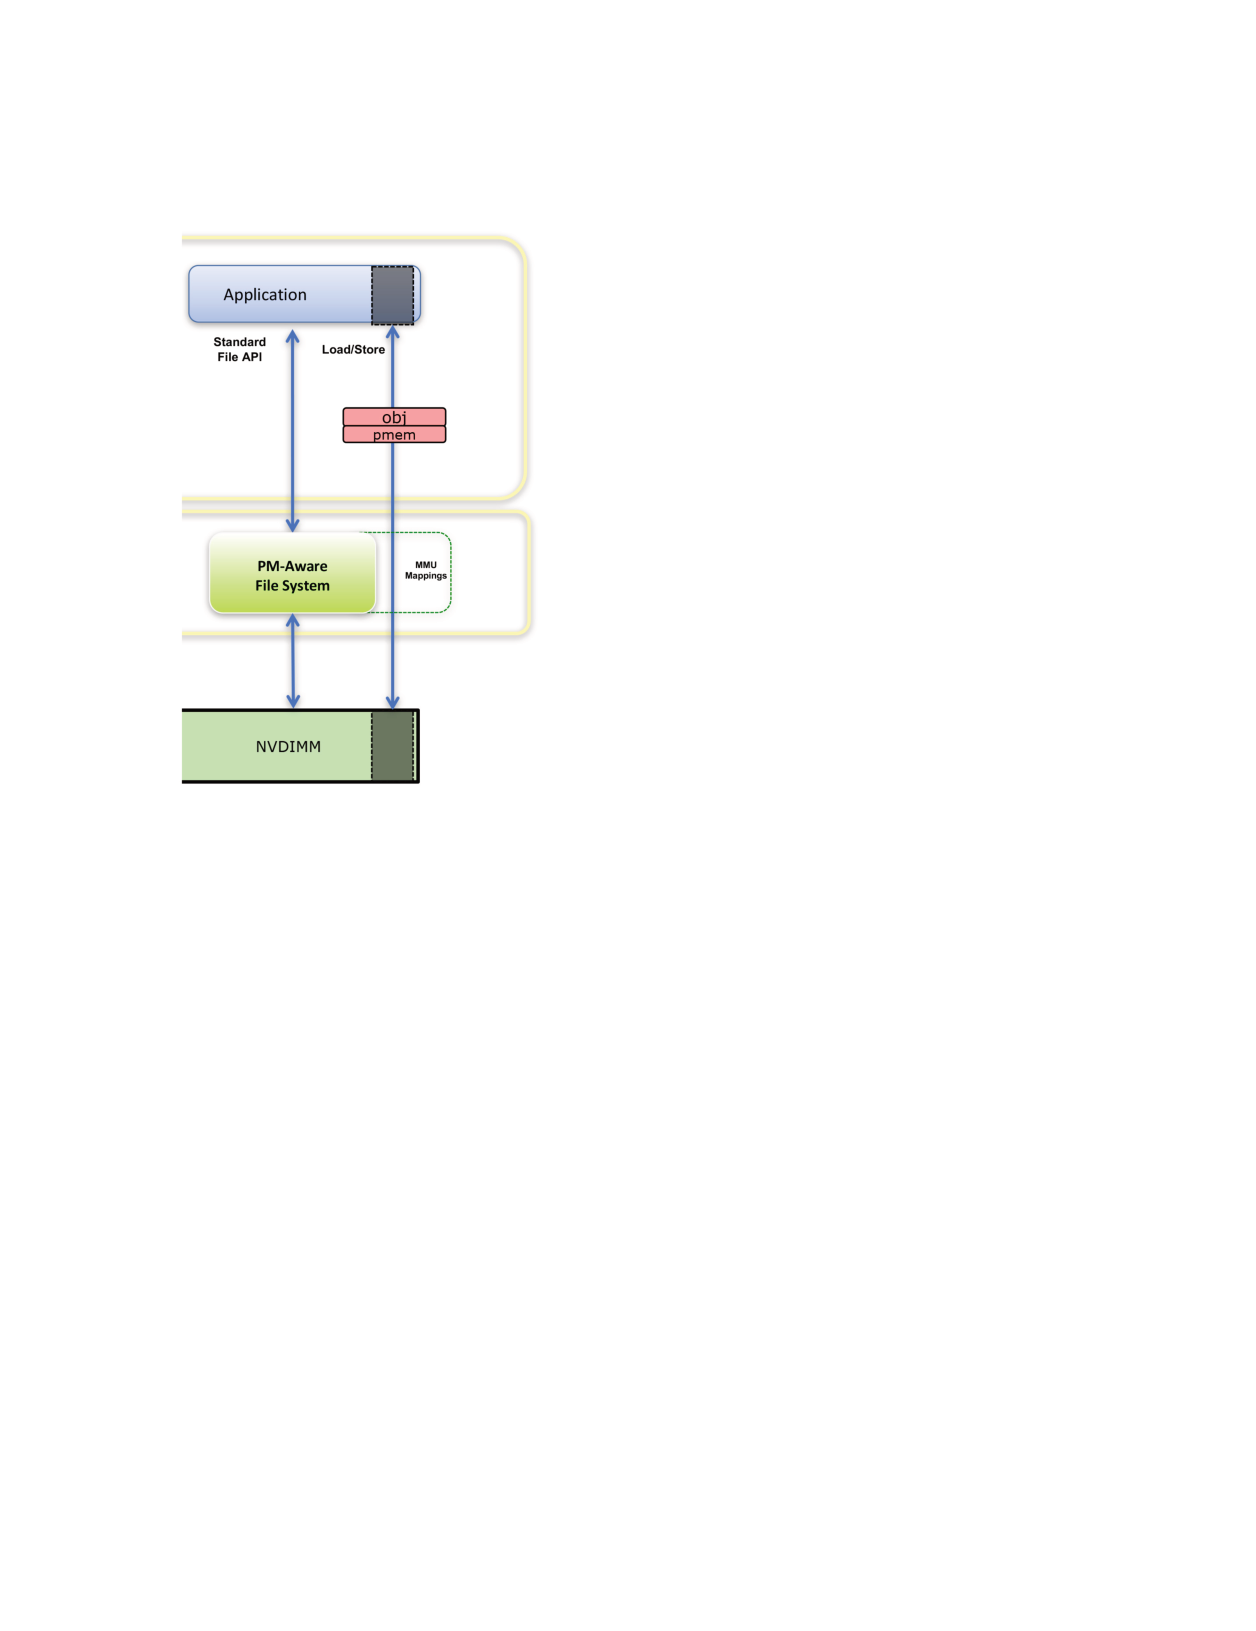
\includegraphics[scale=1]{figures/nvram/pmdk-sys-arch-extract.pdf}
    \caption{System architecture with PMDK to manage NVRAM \cite{rudoff2017persistent}.}
    \label{fig:pmdk-sys}
\end{figure}

Another discussed approach to manage \ac{NVRAM} is through designated file
systems \cite{oukid2017data, andrei2017sap}. File systems provide a well-known
and suitable abstraction for non-volatile storage. In order to enable regular
memory access in a load-store manner, individual files can be mapped into
virtual memory. However, traditional file systems are not directly well-suited
for use with \ac{NVRAM}. One reason is that most operating systems provide a
page cache which is used by file systems to defer expensive disk \ac{IO}. In the
case of \ac{NVRAM}, page caches may be no longer needed, as updates to
\ac{NVRAM} incur far less latency compared to other non-volatile memories. In
this regard, page caches even add overhead instead of mitigating it. Apart from
that, they add a level of indirection which makes writes to \ac{NVRAM} more
likely to be torn by failures. Also, traditional file systems are usually
designed for block-oriented devices which may no longer be the best option.
Therefore, several \ac{NVRAM}-aware file systems have been proposed
\cite{condit2009better, wu2011scmfs, dulloor2014system, xu2016nova}. The key
feature of these file systems is a zero-copy mechanism by circumventing page
caches. This enables true store-load semantics for memory-mapped files. Other
aspects include attempts to leverage the byte-addressable nature of \ac{NVRAM}
and crash-related consistency issues. Yet, there appears to be a growing consensus
that instead of designing new file systems for \ac{NVRAM}, existing file systems
should be outfitted to support \ac{NVRAM}. A prominent result is the adoption of
\ac{DAX} in the Linux kernel \cite{oukid2017data, andrei2017sap,
rudoff2017persistent}. \ac{DAX} is a mechanism to bypass the operating system's
page cache and is used by PMDK \cite{rudoff2017persistent, pmdk2018home}.

% \paragraph{Consistency}
%
% A notorious problem with \ac{NVRAM} is consistency in case of crashes
% \cite{condit2009better, dulloor2014system, oukid2017data}. Due to the complex
% nature of this subject, further discussion is deferred to the next section.
%
% \todo[inline]{fix layout (unfitting page break, remove this paragraph?)}

\subsection{Preserving Consistency}
\label{ch:nvram-consistency}
As pointed out earlier, the consistency of data stored in \ac{NVRAM} is
vulnerable to crashes or power failures \cite{condit2009better,
dulloor2014system, oukid2017data}. Since \ac{NVRAM} is directly attached to the
processor memory interface, there is no need to use techniques such as \ac{DMA}
to transfer a modified page to external storage. This also means that a memory
operation solely relies on the \ac{CPU} which usually gives no confirmation when
that operation completes. In this context, there are two major issues that
threaten the consistency of data written to \ac{NVRAM}, namely out-of-order
execution and deferred write-back.

\subsubsection{Out-Of-Order Execution}

When executing a program, processors fetch instructions in a consecutive manner.
Some instructions may inflict minimal latency, while others such as load
operations may delay further execution for hundreds of cycles. In an attempt to
optimize instruction throughput, individual instructions may be reordered. While
compilers may statically define promising orders, processors are able to reorder
instructions at runtime. This enables processors to optimize resource
utilization and hide latencies of time-consuming instructions. However, only
reorderings that do not violate data dependencies between instructions are
possible. While processors do prevent such conflicts, there are dependencies
that cannot be observed. For example, in order to mark a chunk of data as
durable in \ac{NVRAM}, one might store a designated flag immediately after the
operation completed. With out-of-order execution it is possible that the flag is
written before the payload. This can lead to severe inconsistencies especially
when a crash prevents the chunk from being written.

A common method to counter this issue is to enforce memory order with memory
barriers (also fences) \cite{dulloor2014system, schwalb2016hyrise,
oukid2017data}. A memory barrier prevents the \ac{CPU} from proceeding until all
prior memory operations have completed. Although a barrier does not directly
order its preceding instructions, it can be used to impose an order on separate
sequences of instructions. An example for a memory barrier is \code{sfence} on
x86 architectures. While this approach solves the initial problem, it has a
notable drawback. Memory barriers defeat the purpose of out-of-order execution.
As a result, \ac{CPU} pipelines are likely to stall, hence reducing resource
utilization. Furthermore, store buffers are flushed leading to higher latencies
when accessing data of deferred store operations. Therefore, barriers can have a
significant impact on runtime performance, unless used judiciously. With
\emph{epoch barriers} a similar approach has been proposed to address both order
and durability issues \cite{condit2009better}.

\subsubsection{Deferred Write-Back}

In many modern processor architectures store operations may not immediately
lead to an update in main memory. This behavior can be caused by intermediary
buffers such as memory order buffers, caches, and memory controller buffers.
While their individual purpose may vary, they all defer memory write-back
operations. This is a known vulnerability for consistency in \ac{NVRAM} as the
mentioned buffers are volatile and deferred stores may be lost when power fails
\cite{condit2009better, oukid2017data}. In order to preserve consistency, it is
necessary to force write-back in all of these cases. Figure
\ref{fig:memory-interface} shows a typical memory hierarchy with several layers
by which stores can be deferred.

\begin{figure}[h!]
    \centering
    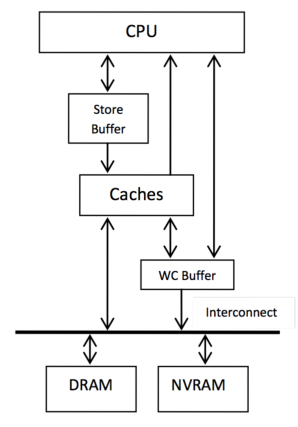
\includegraphics[scale=0.9]{figures/nvram/memory-subsystem.pdf}
    \caption{Architecture of memory subsystem \cite{bhandari2012implications}.}
    \label{fig:memory-interface}
\end{figure}

\paragraph{\acp{MOB}}

In conjunction with instruction scheduling and cache coherency protocols a
memory order buffer may be present. It holds all loads and stores, with the
exception of non-temporal operations. In order to prevent a deferred write-back
through \acp{MOB}, their store buffers must be flushed. On x86
architectures this can be achieved with a store fence operation such as
\code{sfence}. As mentioned above, memory barriers carry a considerable
overhead. However, if memory barriers are already used for enforcing program
order, then flushing store buffers is a desirable side effect and incurs no
overhead.

\paragraph{Caches}

Processor caches help avoid access latencies and reduce memory bus traffic for
frequently used data. A possible exception are non-temporal stores and data
chunks marked as uncacheable. Similar to \acp{MOB}, caches are
volatile so an abrupt power failure may lead to lost updates. The issue with
this is not that updates are lost but that it is unclear which updates are lost,
if any. The reason for this circumstance is the cache eviction policy trying to
compensate for typically narrow cache volume. Depending on policy, cache
content, and system load, a modified chunk may or may not be flushed to main
memory. An application scenario where such behavior is unacceptable is
transactions. In the example in Figure \ref{fig:nvram-cache-crash}, two stores are cached. One store becomes durable because its cache line is evicted, while the other remains in cache and is lost in a crash.

% \todo[inline]{Insert figure showing inconsistency due to crash}

%\begin{lstlisting}
%T1: r(A) w(A) c*   -- Cache ------------------------ (crash)
%T2: -------------- r(A) w(B) c -- Cache -- NVRAM --- (crash)
%\end{lstlisting}

\begin{figure}[!ht]
    \centering
    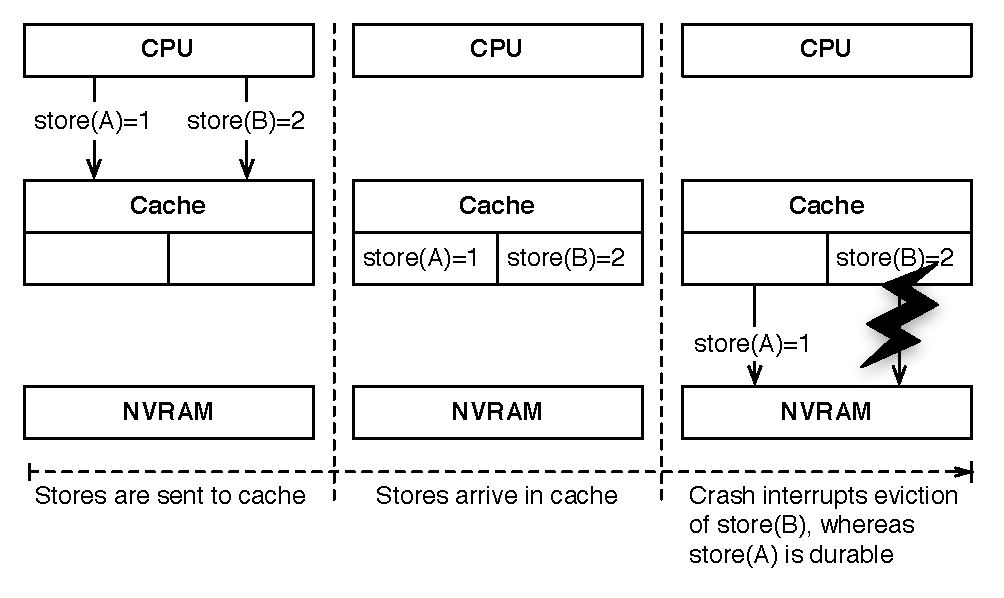
\includegraphics[width=0.70\textwidth]{figures/nvram/cache-crash.pdf}
    \caption{A sitation where only one of two cached stores reaches durability.}
    \label{fig:nvram-cache-crash}
\end{figure}

An approach to prevent such inconsistencies is to disable caching for selected
memory regions but that could introduce considerable overhead for frequently
used data. A more popular approach is to evict cache lines programmatically
whenever necessary \cite{condit2009better, dulloor2014system, oukid2017data}. On
x86 architectures this can be done with the \code{clflush} or \code{clflushopt}
instructions. However, the problem with a cache line flush is that wanting to
make a cache line durable does not always mean that is should be evicted.
Therefore, there are proposals for instructions, such as \code{clwb}, that send
a cache line to a memory controller without evicting it \cite{kolli2016high,
oukid2017data}. Unfortunately, at the time of this writing, there is no evidence
of a processor to implement this instruction.

\paragraph{\acp{WPQ}}

Once a cache line is flushed, it is propagated to a memory controller where it
is buffered in a \ac{WPQ}. Again, the problem is that such a buffer is usually
volatile. This means that a power failure could lead to lost updates to
\ac{NVRAM}. Even though residual power in \ac{DRAM} has been shown to be
substantial, there is no reliable way to ensure a full \ac{WPQ} flush
\cite{halderman2008lest}. This circumstance has given rise to many discussions
in the past \cite{condit2009better, dulloor2014system, kolli2016high}. Some
authors proposed a designated instruction for flushing \acp{WPQ}. An example is
the meanwhile deprecated \code{pcommit} instruction (formerly known as
\code{pm\_wbarrier}) \cite{dulloor2014system, oukid2015instant,
volos2017whisper}. Others have developed more general mechanisms for preserving
consistency in \ac{NVRAM} that also address this issue \cite{condit2009better,
pelley2014memory}. The dotted rectangle in Figure \ref{fig:wpq} indicates the
domain in the memory subsystem that must be protected from power failures.

\begin{figure}[h!]
    \centering
    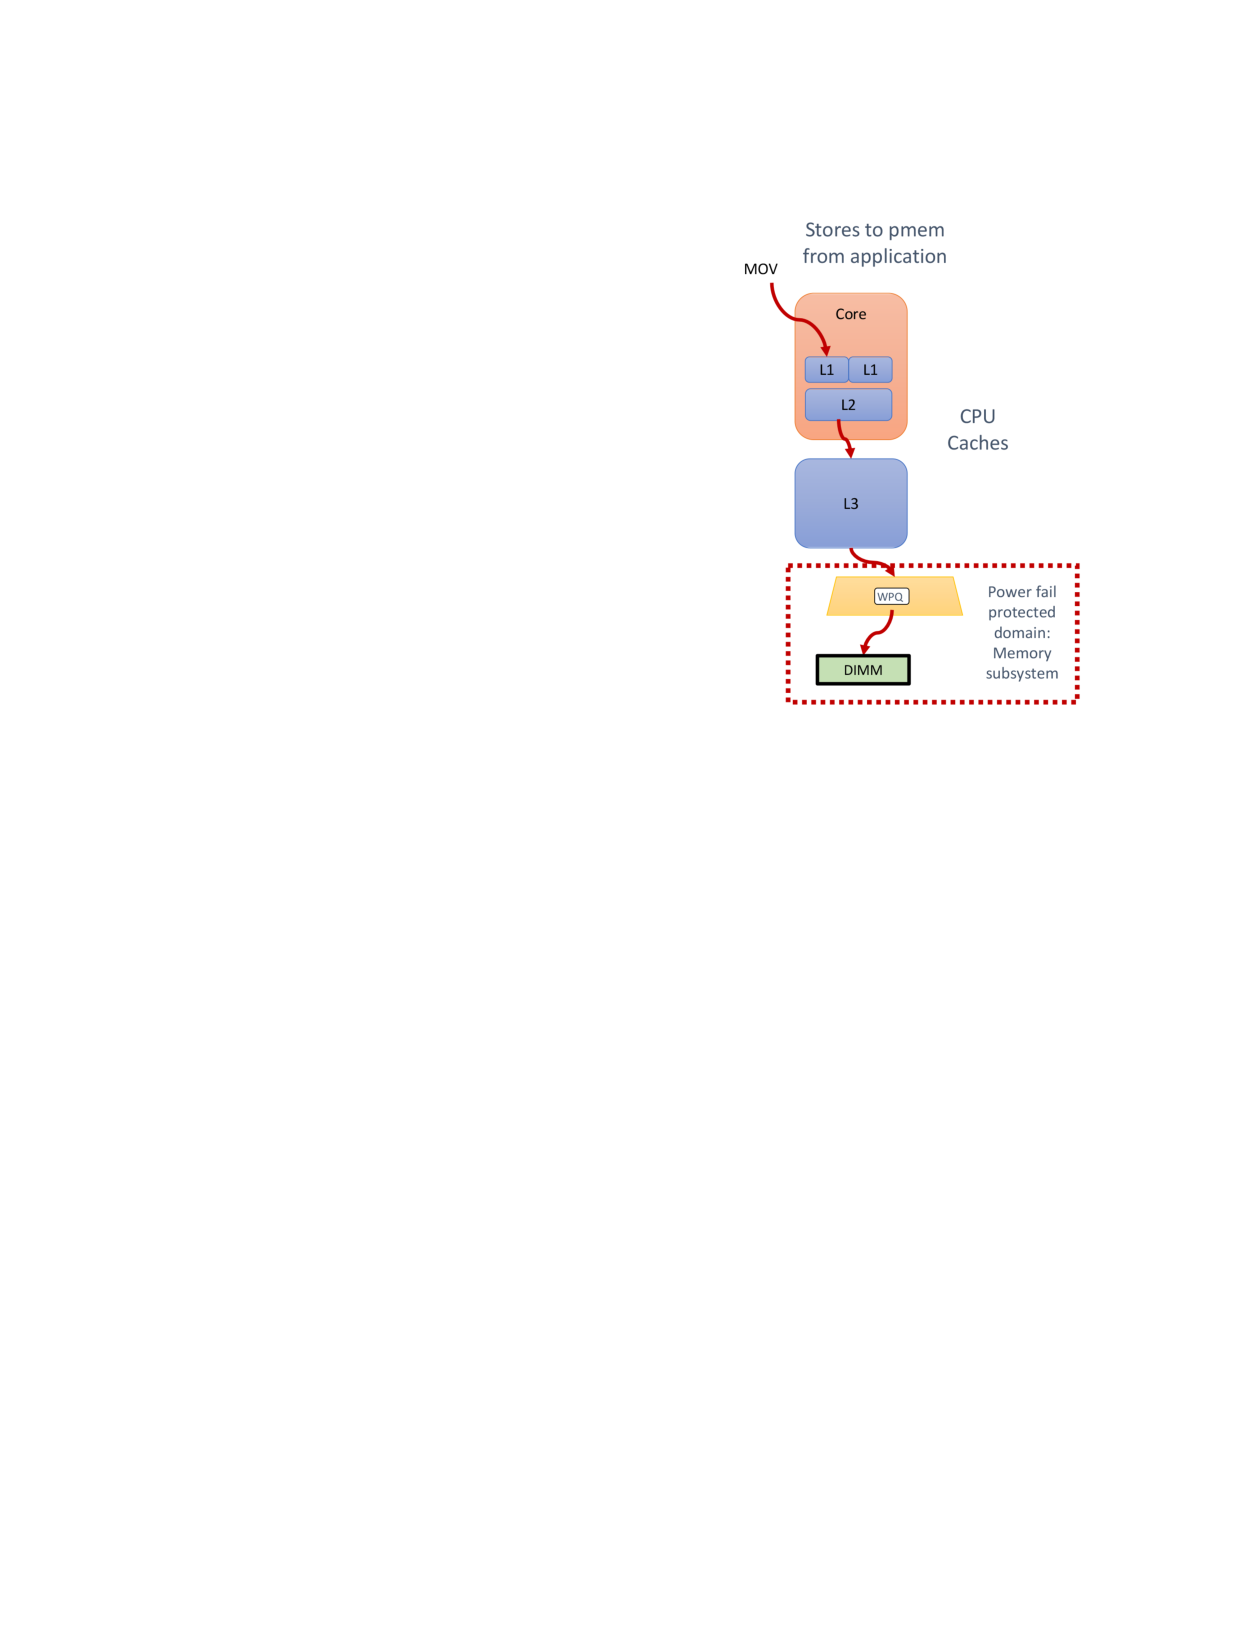
\includegraphics{figures/nvram/adr-example.pdf}
    \captionsetup{justification=centering}
    \caption{The memory domain to be protected against power failures \cite{rudoff2017persistent}.}
    \label{fig:wpq}
\end{figure}

The current state of affairs is that platforms must provide a feature called
\ac{ADR} \cite{volos2017whisper, rudoff2017persistent}. It works by exploiting
the fact that, even in case of a power failure, there is sufficient time and
power to flush \acp{WPQ} in all memory controllers. When the system's power
supply unit detects a power failure, it signals all memory controllers to flush
their \acp{WPQ}. As a result, the programmer does not need to worry about
\acp{WPQ} and no overhead is incurred.

